% Created 2020-02-11 Tue 19:25
% Intended LaTeX compiler: pdflatex
\documentclass[presentation,aspectratio=169,smaller]{beamer}
\usepackage[utf8x]{inputenc}
\usepackage[T1]{fontenc}
\usepackage{graphicx}
\usepackage{grffile}
\usepackage{longtable}
\usepackage{wrapfig}
\usepackage{rotating}
\usepackage[normalem]{ulem}
\usepackage{amsmath}
\usepackage{textcomp}
\usepackage{amssymb}
\usepackage{capt-of}
\usepackage{hyperref}
\usepackage{color}
\usepackage[newfloat]{minted}
\usepackage[utf8]{inputenc}
\usepackage{soul}
\usepackage{unicode-math}
\usepackage{mathtools}
\usepackage[mathletters]{ucs}
\usepackage[cache=false]{minted}
\usemintedstyle{tango}
\setminted{fontsize=\scriptsize}
\setminted{mathescape=true}
\setbeamertemplate{itemize items}[circle]
\setbeamertemplate{enumerate items}[default]
\setlength{\parskip}{\baselineskip}%
\setlength{\parindent}{0pt}%
\setbeamertemplate{navigation symbols}{}%remove navigation symbols
\newcommand{\hlyellow}[1]{\colorbox{yellow!50}{$\displaystyle#1$}}
\newcommand{\hlfancy}[2]{\sethlcolor{#1}\hl{#2}}
\usetheme{default}
\author{Boris Buliga, Valentyn Vakatsiienko}
\date{\today}
\title{Functional Forkshop: Part 1}
\hypersetup{
 pdfauthor={Boris Buliga, Valentyn Vakatsiienko},
 pdftitle={Functional Forkshop: Part 1},
 pdfkeywords={},
 pdfsubject={},
 pdfcreator={Emacs 28.0.50 (Org mode 9.3.4)}, 
 pdflang={English}}
\begin{document}

\maketitle
\newcommand{\mathcolorbox}[2]{%
  \begingroup
  \setlength{\fboxsep}{2pt}%
  \colorbox{#1}{$\displaystyle #2$}%
  \endgroup
}

\AtBeginSection[]{
  \begin{frame}
  \vfill
  \centering
  \begin{beamercolorbox}[sep=8pt,center,shadow=true,rounded=true]{title}
    \usebeamerfont{title}\insertsectionhead\par%
  \end{beamercolorbox}
  \vfill
  \end{frame}
}

\section*{Intro}
\label{sec:orgb919706}
\begin{frame}[label={sec:org2387419}]{About us}
\vspace*{20px}

\begin{block}{Valik}
\begin{columns}
\begin{column}{0.75\columnwidth}
Server guild manager in Kyiv. Formerly forced people to use functional
programming style in the Domains (Premium) team. Now works on Tagless Infra to
provide you with the best tools for your daily needs. Which are all functional,
of course.
\end{column}

\begin{column}{0.25\columnwidth}
\begin{center}
\includegraphics[height=2.5cm]{images/valik.png}
\end{center}

\pause
\end{column}
\end{columns}
\end{block}

\begin{block}{Boris}
\begin{columns}
\begin{column}{0.75\columnwidth}
Developer at Payments by Wix team. Jumps between two extremes - Emacs Lisp and
Haskell. Wants to force people around to use both languages, but fails to
explain why.
\end{column}

\begin{column}{0.25\columnwidth}
\begin{center}
\includegraphics[height=2.5cm]{images/boris.jpg}
\end{center}
\end{column}
\end{columns}
\end{block}
\end{frame}

\begin{frame}[label={sec:org4f6b0a3}]{About the Forkshop}
\begin{itemize}
\item Basic forkshop is split into several parts:
\begin{enumerate}
\item Type classes, Semigroups and Monoids.
\item Functors and Applicative Functors.
\item Selective Applicative Functors and Monads.
\item Readers.
\item Comonads.
\end{enumerate}
\item Theory and practice. Make sure that you are ready to write the code.
\item Target audience is Scala developers learning FP.
\end{itemize}
\end{frame}

\begin{frame}[label={sec:org1a0433d},fragile]{Whys}
 \begin{itemize}
\item <1-> Functional programming roams (a bit).
\begin{itemize}
\item More projects are using functional programming techniques and idioms (at
different scale).
\end{itemize}
\item <2-> Some people are still confused by all these functional talks (\texttt{OptionT}, type
lambdas etc).
\item <3-> Having a common language and understanding of some fundamental stuff is
important.
\end{itemize}
\end{frame}

\section*{Today}
\label{sec:orgc2fb44f}
\begin{frame}[label={sec:orgc78ee08}]{Agenda}
\begin{itemize}
\item Type classes
\item Semigroups
\item Monoids
\item 3 interesting™ tasks
\end{itemize}
\end{frame}

\begin{frame}[label={sec:orgb5ff627},fragile]{Before we start}
 \begin{minted}[]{bash}
$ git clone git@github.com:wax-org/fforkshop-monoids-scala.git
\end{minted}

And import it as sbt project.
\end{frame}

\section{Type classes}
\label{sec:orgce27121}

\begin{frame}[label={sec:org8c1ba42}]{Application definition}
\begin{itemize}
\item We are writing a game.
\item With multiple different creatures.
\item Everyone introduces themselves.
\item Introduction consists of animations and text showing in a bubble.
\end{itemize}
\end{frame}

\begin{frame}[label={sec:orgb7c3c28},fragile]{Meet the hero}
 \begin{minted}[]{scala}
case class Hero(name: String, job: String, level: Int) {
  def introduce(): String = s"Hi! My name is $name. I am $level level $job."
}

object Game extends App {
  val player = Hero("Valik", "Black Mage", 20)

  someRealShitSounds()
  drawBubble(player.introduce())
  someRealShitAnimations()
}

// Hi! My name is Valik. I am 20 level Black Mage.
\end{minted}
\end{frame}

\begin{frame}[label={sec:orgbf0fc6e},fragile]{Every hero needs a monster}
 \begin{minted}[]{scala}
case class Orc(name: String, level: Int) {
  def introduce(): String =
    s"Lok-tar ogar! Me be $name. Me be strong. Level $level strong!"
}

case class Ooze(level: Int) {
  def introduce(): String = 1.to(level).map(_ => "brlup").mkString("-")
}
\end{minted}
\end{frame}

\begin{frame}[label={sec:org9e7f5b3},fragile]{Game}
 \begin{columns}
\begin{column}[t]{0.46\columnwidth}
\begin{minted}[]{scala}
object Game extends App {
  val player = Hero("Valik", "Black Mage", 20)
  val orc = Orc("Garrosh", 105)
  val ooze = Ooze(2)

  // Introduce player
  someRealShitSounds()
  drawBubble(player.introduce())
  someRealShitAnimations()

  // Introduce orc
  someRealShitSounds()
  drawBubble(orc.introduce())
  someRealShitAnimations()

  // Introduce ooze
  someRealShitSounds()
  drawBubble(ooze.introduce())
  someRealShitAnimations()
}

// Hi! My name is Valik. I am 20 level Black Mage.
// Lok-tar ogar! Me be Garrosh. Me be strong. Level 105 strong!
// brlup-brlup
\end{minted}

\pause
\end{column}

\begin{column}[t]{0.46\columnwidth}
\vspace*{0px}

Issues with this code:

\begin{enumerate}
\item Repetition
\item Noise
\end{enumerate}
\end{column}
\end{columns}
\end{frame}

\begin{frame}[label={sec:orgf865e74},fragile]{Introducing abstractions}
 \begin{columns}
\begin{column}[t]{0.5\columnwidth}
\begin{minted}[]{scala}
//



case class Hero(...) {
  def introduce(): String = s"..."
}

case class Orc(...) {
  def introduce(): String = s"..."
}

case class Ooze(...) {
  def introduce(): String = s"..."
}
\end{minted}

\pause
\end{column}

\begin{column}[t]{0.5\columnwidth}
\begin{minted}[]{scala}
trait Introducible {
  def introduce(): String
}

case class Hero(...) extends Introducible {
  override def introduce(): String = s"..."
}

case class Orc(...) extends Introducible {
  override def introduce(): String = s"..."
}

case class Ooze(...) extends Introducible {
  override def introduce(): String = s"..."
}
\end{minted}
\end{column}
\end{columns}
\end{frame}

\begin{frame}[label={sec:orgea818b9},fragile]{Game with trait}
 \begin{columns}
\begin{column}[t]{0.5\columnwidth}
\begin{minted}[]{scala}
def introduce(phrase: String): Unit = {
  someRealShitSounds()
  drawBubble(phrase)
  someRealShitAnimations()
}

object Game extends App {
  /* ... */

  introduce(player.introduce())
  introduce(orc.introduce())
  introduce(ooze.introduce())
}
\end{minted}
\end{column}

\begin{column}[t]{0.5\columnwidth}
\begin{minted}[]{scala}
def introduce(creature: Introducible): Unit = {
  someRealShitSounds()
  drawBubble(creature.introduce())
  someRealShitAnimations()
}

object Game extends App {
  /* ... */

  introduce(player)
  introduce(orc)
  introduce(ooze)
}
\end{minted}
\end{column}
\end{columns}

\pause

\begin{itemize}
\item No more \texttt{introduce(\_.introduce())}.
\item We are adaptive. Less code needs to be changed if we need something new in the
\texttt{introduce} function (e.g. sound name) - just add new 'method' to the trait.
\item Refactoring becomes easier.
\end{itemize}
\end{frame}

\begin{frame}[label={sec:orge018fce},fragile]{Here comes the cockatrice}
 \begin{columns}
\begin{column}{0.55\columnwidth}
\begin{minted}[]{scala}
import io.proprietary.monsters.cockatrice._

/* ... */

object Game extends App {
  /* ... */

  val cockatrice = Cockatrice(
    level = 666,
    element = Element.Fire
  )

  introduce(cockatrice) // ???
                        // ain't gonna work
}
\end{minted}
\end{column}

\begin{column}{0.45\columnwidth}
\begin{center}
\includegraphics[height=5cm]{images/cockatrice.jpg}
\end{center}
\end{column}
\end{columns}
\end{frame}

\begin{frame}[label={sec:org98b9228},fragile]{Shawarma to the rescue}
 \begin{columns}
\begin{column}{0.25\columnwidth}
\begin{center}
\includegraphics[height=7cm]{images/shawarma.jpg}
\end{center}
\end{column}

\begin{column}{0.75\columnwidth}
\begin{minted}[]{scala}
import io.proprietary.monsters.cockatrice._

/* ... */

case class CockatriceWrapper(cockatrice: Cockatrice) extends Introducible {
  override def introduce(): String = {
    import cockatrice._
    s"Haha. I am a ${element.shortName} cockatrice of level ${level}."
  }
}

object Game extends App {
  /* ... */

  val cockatrice = Cockatrice(level = 666, element = Element.Fire)
  val cockatriceW = CockatriceWrapper(cockatrice)

  introduce(cockatriceW)

  /* ... */
}


// Haha. I am a fire cockatrice of level 666.
\end{minted}
\end{column}
\end{columns}
\end{frame}

\begin{frame}[label={sec:orgd045313}]{Calm down and reevaluate our goal}
\begin{itemize}
\item <1-> Abstraction - caring about what you can do and not what you are. E.g.
separation of data and behaviour.
\item <2-> Composition - having a way to express something that can do several things at
once.
\item <3-> Extensibility - extending all kind of types:
\begin{itemize}
\item types we own
\item types we don't own
\item even built-in types
\end{itemize}
\end{itemize}
\end{frame}

\begin{frame}[label={sec:org27501d2},fragile]{\texttt{trait} + wrapper: abstraction}
 Abstraction holds. Proof is the \texttt{introduce} function itself.

\begin{minted}[]{scala}
def introduce(creature: Introducible): Unit = {
  someRealShitSounds()
  drawBubble(creature.introduce())
  someRealShitAnimations()
}
\end{minted}
\end{frame}

\begin{frame}[label={sec:orgc03a233},fragile]{\texttt{trait} + wrapper: composition}
 Composition holds thanks to \texttt{with} keyword.

\pause

\begin{minted}[]{scala}
trait CanAttack {
  def attack(): Unit
}

def patheticAttack[A <: Introducible with CanAttack](creature: A): Unit
\end{minted}

\pause

\texttt{with} keyword is not commutative

\texttt{Introducible with CanAttack} != \texttt{CanAttack with Introducible}.
\end{frame}

\begin{frame}[label={sec:orgd025c0f},fragile]{\texttt{trait} + wrapper: extensibility}
 Extensibility holds, but with several caveats:

\begin{enumerate}
\item No consistency - we wrap only types we don't own.
\item Wrappers don't compose very well. You might even wrap your wrappers.
\item Bad usability:
\begin{enumerate}
\item You can’t interchangeably use wrapper and the underlying value.
\item You can't plug in different behaviour implementations.
\end{enumerate}
\end{enumerate}
\end{frame}

\begin{frame}[label={sec:org199bf21}]{You know where it’s going to, right?}
\pause

\begin{center}
\includegraphics[height=7cm]{images/f_.jpg}
\end{center}
\end{frame}

\begin{frame}[label={sec:org15d8dd0},fragile]{Dividing data and behaviour}
 \begin{columns}
\begin{column}[t]{0.5\columnwidth}
\begin{minted}[]{scala}
trait Introducible {
  def introduce(): String
}

def introduce(creature: Introducible): Unit = {

  /* ... */
  drawBubble(creature.introduce())
  /* ... */
}
\end{minted}

\pause
\end{column}

\begin{column}[t]{0.5\columnwidth}
\begin{minted}[]{scala}
trait Introducible[A] {
  def introduce(a: A): String
}

def introduce[A](creature: A,
                 impl: Introducible[A]): Unit = {
  /* ... */
  drawBubble(impl.introduce(creature))
  /* ... */
}
\end{minted}
\end{column}
\end{columns}
\end{frame}

\begin{frame}[label={sec:orgfc6afa6},fragile]{Usage}
 \begin{minted}[]{scala}
// Define new trait
trait Introducible[A] {
  def introduce(a: A): String
}
\end{minted}

\pause

\begin{minted}[]{scala}
// Remove behaviour from data
case class Hero(name: String, job: String, level: Int)
\end{minted}

\pause

\begin{minted}[]{scala}
// Implement behaviour as a value in companion object
object Hero {
  val introducibleHero: Introducible[Hero] = new Introducible[Hero] {
    override def introduce(a: Hero): String =
      s"..."
  }
}
\end{minted}

\pause

\begin{minted}[]{scala}
// Pass data and behaviour separately
object Game extends App {
  /* ... */
  introduce(
    creature = hero,
    impl = Hero.introducibleHero
  )
}
\end{minted}
\end{frame}

\begin{frame}[label={sec:org8348461},fragile]{External types? Pff\ldots{}}
 \begin{minted}[]{scala}
import io.proprietary.monsters.cockatrice._

// Implement behaviour as a value in an object
object CockatriceInstances {
  val introducibleCockatrice: Introducible[Cockatrice] = new Introducible[Cockatrice] {
    override def introduce(a: Cockatrice): String =
      s"..."
  }
}
\end{minted}

\pause

\begin{minted}[]{scala}
// Pass data and behaviour separately
object Game extends App {
  /* ... */
  introduce(
    creature = cockatrice,
    impl = CockatriceInstances.introducibleCockatrice
  )
}
\end{minted}
\end{frame}

\begin{frame}[label={sec:orgd4817c2}]{But passing implementation around is\ldots{}}
\begin{center}
\includegraphics[height=5cm]{images/cucumber.jpg}
\end{center}

Cucumbersome
\end{frame}

\begin{frame}[label={sec:orgf5bd285},fragile]{So implicits :(}
 \begin{columns}
\begin{column}[t]{0.5\columnwidth}
\begin{minted}[]{scala}
object Hero {
  val introducibleHero:
      Introducible[Hero] = ???
}

object CockatriceInstances {
  val introducibleCockatrice:
      Introducible[Cockatrice] = ???
}

def introduce[A](creature: A,
                 impl: Introducible[A]): Unit = {
  /* ... */
  drawBubble(impl.introduce(creature))
  /* ... */
}

object Game extends App {
  /* ... */
  introduce(hero, introducibleHero)
  introduce(cockatrice, introducibleCockatrice)
}
\end{minted}

\pause
\end{column}

\begin{column}[t]{0.5\columnwidth}
\begin{minted}[]{scala}
object Hero {
  implicit val introducibleHero:
      Introducible[Hero] = ???
}

object CockatriceInstances {
  implicit val introducibleCockatrice:
      Introducible[Cockatrice] = ???
}

def introduce[A](creature: A)
             (implicit impl: Introducible[A]): Unit = {
  /* ... */
  drawBubble(impl.introduce(creature))
  /* ... */
}

object Game extends App {
  /* ... */
  introduce(hero)
  introduce(cockatrice)
}
\end{minted}
\end{column}
\end{columns}
\end{frame}

\begin{frame}[label={sec:orge9e5c2d},fragile]{Summoning the summoner}
 \begin{columns}
\begin{column}[t]{0.5\columnwidth}
\begin{minted}[]{scala}
trait Introducible[A] {
  def introduce(a: A): String
}






def introduce[A](creature: A)
             (implicit impl: Introducible[A]): Unit = {
  /* ... */
  drawBubble(impl.introduce(creature))
  /* ... */
}
\end{minted}

\pause
\end{column}

\begin{column}[t]{0.5\columnwidth}
\begin{minted}[]{scala}
trait Introducible[A] {
  def introduce(a: A): String
}

object Introducible {
  def apply[A: Introducible]: Introducible[A] =
    implicitly[Introducible[A]]
}

def introduce[A: Introducible](creature: A): Unit = {

  /* ... */
  drawBubble(Introducible[A].introduce(creature))
  /* ... */
}
\end{minted}
\end{column}
\end{columns}
\end{frame}

\begin{frame}[label={sec:org11777ee}]{What have we done?}
\alert{Type class} is just a construct that supports \alert{ad hoc polymorphism}. E.g.
allows one to define polymorphic functions that can be applied to arguments of
different types and behave differently based the type of the arguments.

In other words, \alert{type classes} are solution for supporting \alert{function
overloading}.

\pause

In Scala this can be achieved in several ways:

\begin{itemize}
\item Class inheritance or traits.
\item Type classes (traits + implicits).
\end{itemize}
\end{frame}

\begin{frame}[label={sec:org0fc88c1},fragile]{Type classes: abstraction}
 Abstraction holds. Proof is the \texttt{introduce} function itself.

\pause

\begin{columns}
\begin{column}[t]{0.5\columnwidth}
\begin{minted}[]{scala}
def introduce(creature: Introducible): Unit = {
  /* ... */
  drawBubble(creature.introduce())
  /* ... */
}
\end{minted}
\end{column}

\begin{column}[t]{0.5\columnwidth}
\begin{minted}[]{scala}
def introduce[A: Introducible](creature: A): Unit = {
  /* ... */
  drawBubble(Introducible[A].introduce(creature))
  /* ... */
}
\end{minted}

\pause
\end{column}
\end{columns}

We gain literal data and behaviour separation.
\end{frame}

\begin{frame}[label={sec:orgabb810b},fragile]{Type classes: composition}
 Composition holds. We just pass two different behaviours.

\pause

\begin{minted}[]{scala}
def patheticAttack[A <: Introducible with CanAttack](creature: A): Unit
\end{minted}

\pause

\begin{minted}[]{scala}
def patheticAttack[A : Introducible : CanAttack](creature: A): Unit
def patheticAttack[A](creature: A)
                  (implicit introducibleImpl: Introducible[A],
                   canAttackImpl: CanAttack[A]): Unit
\end{minted}

\pause

But with type classes we don't care about the order.
\end{frame}

\begin{frame}[label={sec:org82485c5}]{Type classes: extensibility}
Extensibility holds with some gains:

\begin{enumerate}
\item Consistency - we treat our own type the same way we treat external types.
\item Usability - no wrappers, no interchangeability problem.
\end{enumerate}
\end{frame}

\begin{frame}[label={sec:org42a1ccc}]{Type classes: final thoughts}
\begin{enumerate}
\item Simple idea giving us good properties.
\item Found a good use for controversial implicits feature.
\item Literal separation of data and behaviour.
\item Good for overloading.
\item + more abstraction, - more code
\end{enumerate}
\end{frame}

\section{Semigroup}
\label{sec:org7b7b7be}

\begin{frame}[label={sec:org6b9510c},fragile]{Time for a quiz!}
 \begin{columns}
\begin{column}[t]{0.5\columnwidth}
What is common between:

\begin{enumerate}
\item \texttt{Int}
\item \texttt{String}
\item \texttt{List}
\item \texttt{PartialFunction}
\item \texttt{HttpMapping}
\end{enumerate}

\pause
\end{column}

\begin{column}[t]{0.5\columnwidth}
They can be combined!

\begin{enumerate}
\item Int + Int = Int
\item String + String = String
\item List ::: List = List
\item PartialFunction orElse PartialFunction = PartialFunction
\item HttpMapping + HttpMapping = HttpMapping
\end{enumerate}
\end{column}
\end{columns}
\end{frame}

\begin{frame}[label={sec:orge20b04b}]{Associativity}
\begin{enumerate}
\item \(Int + Int + Int = Int + (Int + Int) = (Int + Int) + Int\)
\item \(String + String + String = String + (String + String) = (String + String) + String\)
\item etc\ldots{}
\end{enumerate}
\end{frame}

\begin{frame}[label={sec:orgc1328c8}]{Semigroup}
\alert{Semigroup} is a set \(S\) with binary closed operation \(\cdot : S \times S
\rightarrow S\) that satisfies associativity property:

$$\forall a, b, c \in S : (a \cdot b) \cdot c = a \cdot (b \cdot c)$$

Operation is closed when \(\forall a, b \in S : a \cdot b \in S\).
\end{frame}

\begin{frame}[label={sec:org194f538},fragile]{But it’s not that scary}
 \begin{columns}
\begin{column}{0.5\columnwidth}
\begin{minted}[]{scala}
package object typeclass {

  //
  // Laws:
  //   1. $\forall a, b, c \in A: (a \cdot b) \cdot c = a \cdot (b \cdot c)$
  //
  trait Semigroup[A] {
    def combine(x: A, y: A): A
  }

  object Semigroup {
    def apply[A: Semigroup]: Semigroup[A] =
      implicitly[Semigroup[A]]
  }

}
\end{minted}

\pause

In simple words, semigroup is a set with means of combining elements of that
set.

\pause
\end{column}

\begin{column}{0.5\columnwidth}
\begin{center}
\includegraphics[height=7cm]{images/scary.png}
\end{center}
\end{column}
\end{columns}
\end{frame}

\begin{frame}[label={sec:orga2c38e5}]{Important!}
Semigroup is a pair of the set and the operation.

You can’t say that string is a semigroup, you must provide an operation.

And in many cases there is more than one operation for a set to form a
semigroup.
\end{frame}

\begin{frame}[label={sec:org9878cee},fragile]{What is law?}
 \begin{itemize}
\item <1-> In programming world it's just a contract.
\item <2-> Operations in the type classes are very generic.
\begin{minted}[]{scala}
def combine(x: A, y: A): A
\end{minted}
\item <3-> So type classes should have some associated laws.
\item <4-> Laws describe properties of these operations and connection between operations
in one type class.
\item <5-> Contract of the interface gives us confidence when we write generic code.
\item <6-> And as you will see, we really care about these laws.
\end{itemize}
\end{frame}

\begin{frame}[label={sec:orgfb9da92},fragile]{Instance example}
 \begin{minted}[]{scala}
package object implicits {
  implicit val stringSemigroup: Semigroup[String] = new Semigroup[String] {
    override def combine(x: String, y: String): String = x + y
  }
}
\end{minted}
\end{frame}

\begin{frame}[label={sec:org1990d43},fragile]{Checking laws - \sout{pen and paper} in comments}
 \begin{minted}[]{scala}
package object implicits {
  implicit val stringSemigroup: Semigroup[String] = new Semigroup[String] {
    override def combine(x: String, y: String): String = x + y
  }
}

/*
combine(a, combine(b, c))
  = combine(a, b + c)
  = a + (b + c)
  = (associativity of +)
  = (a + b) + c = combine(a + b, c)
  = combine(combine(a, b), c)
*/
\end{minted}
\end{frame}

\begin{frame}[label={sec:org96d2403}]{You're developer after all}
\begin{center}
\includegraphics[height=7cm]{images/you-re-programmer.jpg}
\end{center}
\end{frame}

\begin{frame}[label={sec:orgb7da609},fragile]{Question on the interview: property based testing}
 \begin{minted}[]{scala}
object SemigroupSpecification extends Properties("Semigroup") with SemigroupSpecificationSupport {
 include(semigroup[String](stringSemigroup))
}

trait SemigroupSpecificationSupport {
 def semigroup[A](sg: Semigroup[A])(implicit ar: Arbitrary[A], tag: ClassTag[A]): Properties =
   new Properties(s"Semigroup[${tag.toString}]") {


     // $\forall a, b, c \in A: (a \cdot b) \cdot c = a \cdot (b \cdot c)$
     property("associativity") = forAll { (a: A, b: A, c: A) =>
       sg.combine(sg.combine(a, b), c) =? sg.combine(a, sg.combine(b, c))
     }


   }
}

/*
+ Semigroup.Semigroup[java.lang.String].associativity: OK, passed 100 tests
  .
*/
\end{minted}
\end{frame}

\begin{frame}[label={sec:org329ea89},fragile]{More than one valid instance}
 \begin{minted}[]{scala}
package object implicits {
  implicit val stringSemigroup: Semigroup[String] = new Semigroup[String] {
    override def combine(x: String, y: String): String = x
  }
}
\end{minted}
\end{frame}

\begin{frame}[label={sec:org9a38f1e}]{More examples}
\begin{itemize}
\item Numbers with \(+\), \(*\), \(min\), \(max\)
\item Booleans with conjunction, disjunction, implication etc.
\item Square nonnegative matrices with multiplication.
\item Lists, Strings, Maps etc. with concatenation/union
\item We will see even more examples during practical part.
\end{itemize}
\end{frame}

\begin{frame}[label={sec:org21cec5a}]{Contra-examples}
\begin{itemize}
\item \(\{\mathbb{N}, /\}\) is not a Semigroup, because \(/\) is not associative.
\item The same goes for \(\{\mathbb{N}, a^b \}\).
\item \(\{\mathbb{N}, -\}\) is not a Semigroup, because \(-\) is not a closed operation,
e.g. \(\exists a, b \in \mathbb{N}: a - b \notin \mathbb{N}\),
for example \(10 - 15 = -5 \notin \mathbb{N}\).
\end{itemize}
\end{frame}

\begin{frame}[label={sec:orgbd435af},fragile]{Coding time}
 \begin{enumerate}
\item <1-> Go to \texttt{src/main}
\item <2-> Task 1
\begin{enumerate}
\item Implement missing \texttt{Semigroup} instances in
\texttt{wax.typeclass.semigroup.cats.implicits}
\item Run \texttt{wax.typeclass.semigroup.laws.cats.SemigroupSpec}
\end{enumerate}
\item <3-> Task 2
\begin{enumerate}
\item Implement missing \texttt{Semigroup} instances in
\texttt{wax.typeclass.semigroup.manual.implicits}
\item Run \texttt{wax.typeclass.semigroup.laws.manual.SemigroupSpec}
\end{enumerate}
\end{enumerate}
\end{frame}

\section{Monoid}
\label{sec:org30b4f76}

\begin{frame}[label={sec:org995079f}]{Monoid}
\begin{itemize}
\item Sometimes you want to compose \(n\) elements where \(n \geq 0\).
\item Semigroup works only for \(n > 0\).
\item We need a default element to use if \(n = 0\).
\end{itemize}
\end{frame}

\begin{frame}[label={sec:orge39f5d0}]{Monoid}
One does not simply become a default element:

\begin{itemize}
\item \(Int + 0 = 0 + Int = Int\)
\item \(String + "" = "" + String = String\)
\item etc\ldots{}
\end{itemize}
\end{frame}

\begin{frame}[label={sec:org7e2cf68}]{Monoid}
Back to fancy words.

\pause

A monoid is a set \(S\) with binary closed operation \(\cdot : S \times S
\rightarrow S\) that satisfies associativity property:
$$\forall a, b, c \in S : (a \cdot b) \cdot c = a \cdot (b \cdot c)$$

and identity element \(e\) that satisfies
$$\forall a \in S : e \cdot a = a \cdot e = a$$

Operation is closed when \(\forall a, b \in S : a \cdot b \in S\).

\pause

In other words, monoid is just a semigroup with identity element.
\end{frame}

\begin{frame}[label={sec:orgf5b111a},fragile]{Again, it's not that scary}
 \begin{minted}[]{scala}
package object typeclass {

  //
  // Laws:
  //   1. $\forall a, b, c \in S : (a \cdot b) \cdot c = a \cdot (b \cdot c)$
  //   2. $\forall a \in S : e \cdot a = a \cdot e = a$
  //
  trait Monoid[A] extends Semigroup[A] {
    def empty: A
  }

  object Monoid {
    def apply[A: Monoid]: Monoid[A] = implicitly[Monoid[A]]
  }

}
\end{minted}
\end{frame}

\begin{frame}[label={sec:org5dc2e12},fragile]{Examples}
 \begin{itemize}
\item \(\{\mathbb{N}_0, +\}\), where \(0\) is the identity element.
\item \(\{\mathbb{N}, *\}\), where \(1\) is the identity element.
\item Boolean with XOR, XNOR, OR, AND.
\item String with concatenation (empty string is identity element).
\end{itemize}

\pause

But not every Semigroup forms a Monoid (we are not talking about free monoids
here):

\begin{itemize}
\item \texttt{BigNumber} practically doesn’t have identity element for \texttt{min}.
\end{itemize}
\end{frame}

\begin{frame}[label={sec:orgb078a66}]{Commutativity}
\begin{itemize}
\item <1-> Semigroup and Monoid doesn't require operation to be commutative.
\begin{gather*}
  \neg(\forall a, b \in S : a \cdot b = b \cdot c) \\
  \exists a, b \in S : a \cdot b \ne b \cdot c
\end{gather*}

\item <2-> Examples of non-commutative operations:
\begin{itemize}
\item Arithmetic operations likes \(a - b\), \(a^b\).
\item Diagram drawing.
\item Combining blocks in Minecraft™ (as shown by Tim Williams).
\end{itemize}

\item <3-> Order matters.
\end{itemize}
\end{frame}

\begin{frame}[label={sec:orgb67e4b1}]{The most important question}
\pause

\begin{center}
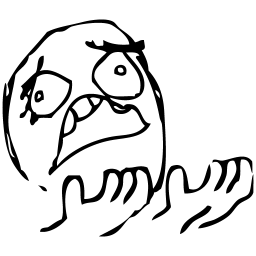
\includegraphics[height=5cm]{images/whyyy.png}
\end{center}

Why did we learn this?
\end{frame}

\section{Fibonacci}
\label{sec:org1ac79e0}

\begin{frame}[label={sec:orgb3f9c5d}]{The Fibonacci numbers}
\begin{align*}
  F_0 &= 0 \\
  F_1 &= 1 \\
  F_n &= F_{n - 1} + F_{n - 2}, \forall n > 1 \\
\end{align*}
\end{frame}

\begin{frame}[label={sec:org5aa42eb},fragile]{Solution}
 \begin{columns}
\begin{column}[t]{0.5\columnwidth}
\begin{block}{What we expect}
\begin{minted}[]{scala}
def fib(n: Int): Int = {
  def fibTail(n: Int, a: Int, b: Int): Int = n match {
    case 0 => a
    case _ => fibTail(n - 1, b, a + b)
  }

  fibTail(n, 0, 1)
}
\end{minted}

\pause
\end{block}
\end{column}

\begin{column}[t]{0.5\columnwidth}
\begin{block}{Ideal solution}
\begin{align*}
  F_n &= \frac {\phi ^ n - {(- \phi)}^{-n}} {\sqrt{5}} \\
  &= \frac {\phi ^ n - {(- \phi)}^{-n}} {2\phi - 1} \\
  \\
  \phi &= \frac {1 + \sqrt{5}}{2}
\end{align*}

\pause
\end{block}
\end{column}
\end{columns}

As they say, truth is somewhere in the logarithm.
\end{frame}

\begin{frame}[label={sec:org7c07f93},fragile]{Two folds}
 \begin{minted}[]{scala}
def foldl[A, B](xs: Seq[A])(z: B)(op: B => A => B): B
\end{minted}

\pause

\begin{columns}
\begin{column}{0.5\columnwidth}
\begin{gather*}
  + : B \rightarrow A \rightarrow B\\
  (((z + x1) + x2) + x3) + x4
\end{gather*}
\end{column}

\begin{column}{0.5\columnwidth}
\begin{center}
\includegraphics[height=6cm]{diag/out/foldl-tree.png}
\end{center}
\end{column}
\end{columns}
\end{frame}

\begin{frame}[label={sec:orgd37f978},fragile]{Two folds}
 \begin{minted}[]{scala}
def foldr[A, B](xs: Seq[A])(z: B)(op: A => B => B): B
\end{minted}

\begin{columns}
\begin{column}{0.5\columnwidth}
\begin{gather*}
  + : A \rightarrow B \rightarrow B\\
  x1 + (x2 + (x3 + (x4 + z)))
\end{gather*}
\end{column}

\begin{column}{0.5\columnwidth}
\begin{center}
\includegraphics[height=6cm]{diag/out/foldr-tree.png}
\end{center}
\end{column}
\end{columns}
\end{frame}

\begin{frame}[label={sec:orgb2096fe},fragile]{Two folds}
 \begin{itemize}
\item \texttt{def foldl[A, B](xs: Seq[A])(z: B)(op: B => A => B): B}
\item \texttt{def foldr[A, B](xs: Seq[A])(z: B)(op: A => B => B): B}
\item Since combining function is asymmetrical in its types:
\begin{itemize}
\item It’s impossible to place parentheses in the arbitrary fashion or even just
change the direction of the \texttt{fold}
\item It’s impossible to implement a total \texttt{fold} without default value of type \texttt{B}
\end{itemize}
\end{itemize}
\end{frame}

\begin{frame}[label={sec:org4edc33a}]{Two folds}
\begin{columns}
\begin{column}[t]{0.5\columnwidth}
\begin{block}{foldl}
$$+ : B \rightarrow A \rightarrow B$$
$$(((z + x1) + x2) + x3) + x4$$

\begin{center}
\includegraphics[height=5cm]{diag/out/foldl-tree.png}
\end{center}
\end{block}
\end{column}

\begin{column}[t]{0.5\columnwidth}
\begin{block}{foldr}
$$+ : A \rightarrow B \rightarrow B$$
$$x1 + (x2 + (x3 + (x4 + z)))$$

\begin{center}
\includegraphics[height=5cm]{diag/out/foldr-tree.png}
\end{center}
\end{block}
\end{column}
\end{columns}
\end{frame}

\begin{frame}[label={sec:orgf238b29},fragile]{What Monoid gives us}
 \begin{itemize}
\item <1-> Combining function is symmetrical (\texttt{combine : A -> A -> A}).
\item <2-> Identity element of type \texttt{A} (\texttt{empty}).
\item <3-> So we can define a special \texttt{fold}
\begin{itemize}
\item \texttt{def foldMonoid[A: Monoid](xs: Seq[A]): A}
\end{itemize}
\item <4-> Identity law says that we can place identity element anywhere.
\item <5-> Associativity law says that we can put parentheses in an arbitrary fashion.
\end{itemize}
\end{frame}

\begin{frame}[label={sec:org7efa268}]{Power in terms of Monoid}
In some cases all elements of the list are the same.

\pause
\begin{equation*}
  a + (a + (a + \ldots + a) \ldots ) = a ^ n
\end{equation*}

\pause

Since we can reorder the parentheses, we can arrange them like this.

\pause

\begin{center}
\includegraphics[height=4cm]{.dot/fold-power-1.png}
\end{center}
\end{frame}

\begin{frame}[label={sec:org9dcdd67}]{Power in terms of Monoid}
\begin{center}
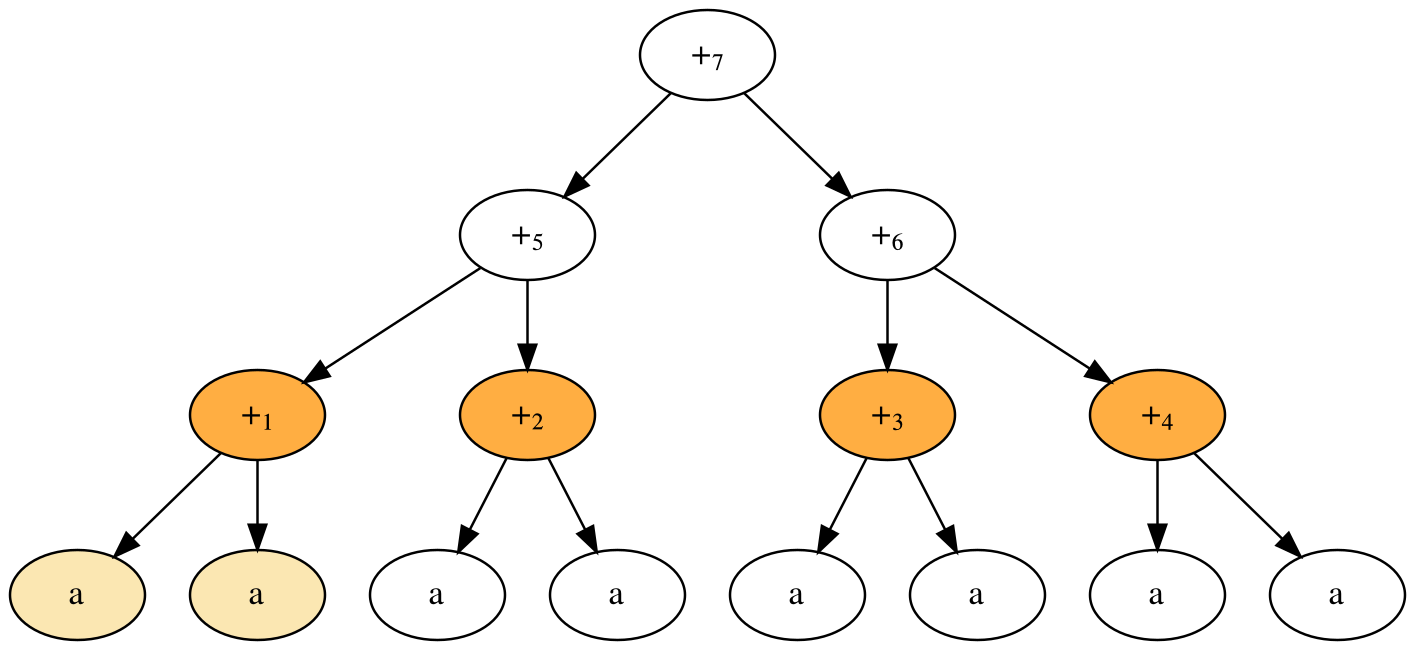
\includegraphics[height=4cm]{.dot/fold-power-2.png}
\end{center}

Evaluating \(a + a\) always yields the same result. So there is no point in
repeating this calculation 4 times.
\end{frame}

\begin{frame}[label={sec:orga25545b}]{Power in terms of Monoid}
\begin{center}
\includegraphics[height=4cm]{.dot/fold-power-3.png}
\end{center}

The same thing with the upper level. In this particular example, we can avoid 4
operations out of 7. In general, this optimisation leads to the result in \(\log
n\) operations.
\end{frame}

\begin{frame}[label={sec:orgd6813d1},fragile]{Power in terms of Monoid}
 All this means that we can define a function \texttt{exp}:

\begin{minted}[]{scala}
def exp[A: Monoid](a: A, n: Int): A = {
  ???
}
\end{minted}
\end{frame}

\begin{frame}[label={sec:orgb9db69a}]{Back to Fibonacci}
Fibonacci number can be calculated in a different way.

\begin{equation*}
  \begin{pmatrix}
    F_{n+1} & F_n \\
    F_n & F_{n-1}
  \end{pmatrix} =
  \begin{pmatrix}
    1 & 1 \\
    1 & 0
  \end{pmatrix} ^ n
\end{equation*}

\pause

\begin{equation*}
  \begin{pmatrix}
    F_4 & F_3 \\
    F_3 & F_2
  \end{pmatrix} =
  \begin{pmatrix}
    1 & 1 \\
    1 & 0
  \end{pmatrix} ^ 3 =
  \begin{pmatrix}
    2 & 1 \\
    1 & 1
  \end{pmatrix} \cdot
  \begin{pmatrix}
    1 & 1 \\
    1 & 0
  \end{pmatrix} =
  \begin{pmatrix}
    3 & 2 \\
    2 & 1
  \end{pmatrix}
\end{equation*}

\pause

\begin{equation*}
  F_3 = 2
\end{equation*}
\end{frame}

\begin{frame}[label={sec:orgea53f00}]{Back to Fibonacci}
\begin{equation*}
  \begin{pmatrix}
    F_{n+1} & F_n \\
    F_n & F_{n-1}
  \end{pmatrix} =
  \begin{pmatrix}
    1 & 1 \\
    1 & 0
  \end{pmatrix} ^ n
\end{equation*}

\pause

\begin{itemize}
\item The Fibonacci number can be calculated using square nonnegative matrix
multiplication.
\item Square nonnegative matrices form Monoid with multiplication.
\item So we can put parentheses in a way we like it.
\end{itemize}
\end{frame}

\begin{frame}[label={sec:org457da9b},fragile]{Coding time}
 \begin{itemize}
\item Open \texttt{wax.exercise.fibonacci.Main} object.
\begin{itemize}
\item \texttt{Main} runs two implementations and profiles them.
\item \texttt{Fib} contains implementation of tailrec and matrix approaches.
\end{itemize}
\item Implement monoid for \texttt{Matrix2x2} in the \texttt{Fib} object.
\item Run \texttt{MatrixSpec} to test your instance.
\item Implement \texttt{exp} function.
\item Run \texttt{FibSpec} to test implementation of \texttt{Fib}.
\item Run \texttt{Main} to see performance differences by yourself.
\end{itemize}

\pause

\begin{equation*}
  a^n = \begin{cases} a(a^2)^{\frac{n-1}{2}}, & \mbox{if } n\mbox{ is odd} \\ (a^2)^{\frac{n}{2}}, & \mbox{if } n\mbox{ is even} \end{cases}
\end{equation*}
\end{frame}

\begin{frame}[label={sec:orgc3014c7}]{Profiling results}
\begin{center}
\begin{tabular}{rrr}
N & Matrix & Tailrec\\
\hline
10 & 60 & 0\\
100 & 0 & 0\\
1000 & 1 & 1\\
10000 & 5 & 6\\
100000 & 46 & 168\\
1000000 & 888 & 15211\\
10000000 & 11266 & -\\
\end{tabular}
\end{center}
\end{frame}

\begin{frame}[label={sec:org4212160},fragile]{Outcome}
 \begin{itemize}
\item <1-> Just think about it.
\item <2-> Giving any monoid we have a helper function that efficiently calculates \(a^n\).
\item <3-> This is only possible because of the \alert{laws} that come with operations.
\item <4-> \texttt{combine} by itself is not interesting, it's too generic.
\item <5-> Laws give us \alert{properties}. Which we use to get a solution that works for
everything that is \texttt{Monoid}.
\item <6-> Monoids are everywhere around us. We deal with them every day, without
even noticing it. Did you expect us to solve Fibonacci using \texttt{Monoid}?
\item <7-> You forgot how matrix multiplication works, but now you remember, right?
\end{itemize}
\end{frame}

\section{Books}
\label{sec:org5011007}

\begin{frame}[label={sec:orgf5287e8}]{Folds with Monoids}
\begin{itemize}
\item We already know that Monoids give us an ability to place parentheses in any
fashion.
\item We already saw that when it comes to folding the list of the same elements we
gain performance.
\item But what if the elements are not equal? Do we gain anything?
\end{itemize}

\pause
\begin{center}
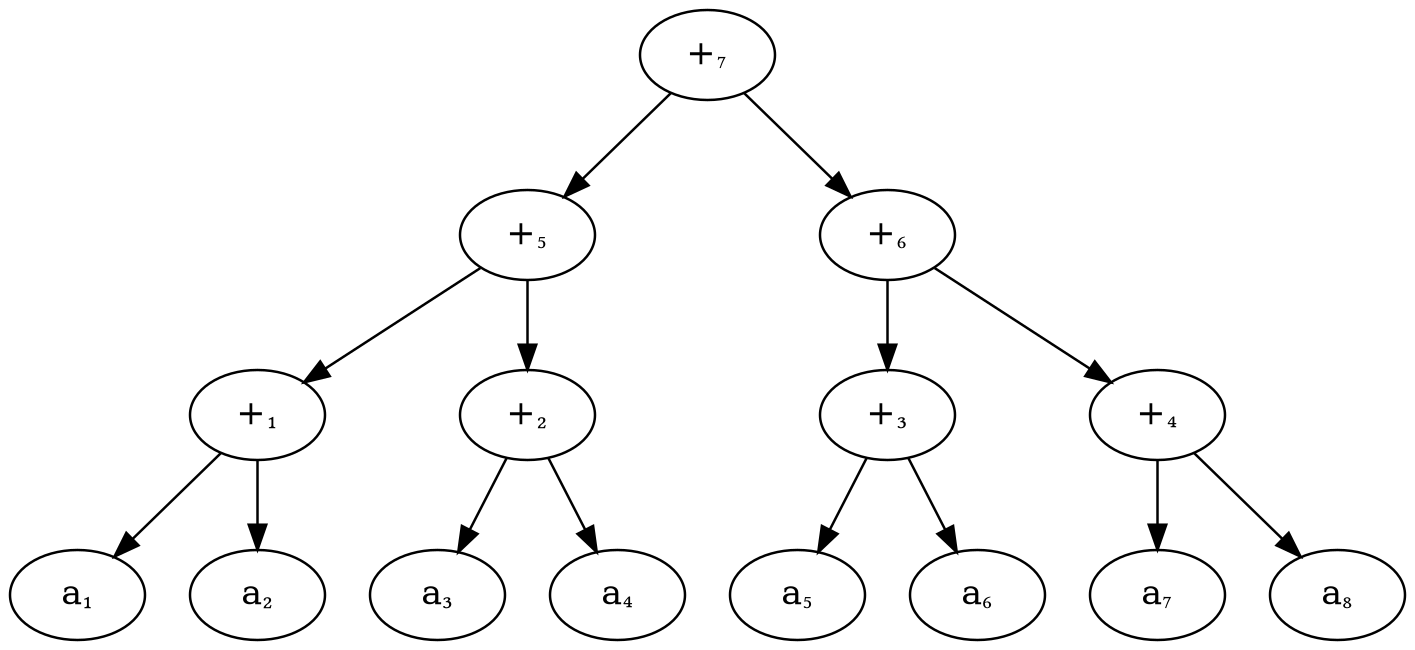
\includegraphics[height=4cm]{.dot/fold-parallel-1.png}
\end{center}
\end{frame}

\begin{frame}[label={sec:org243cdf8}]{Folds with Monoids}
\begin{center}
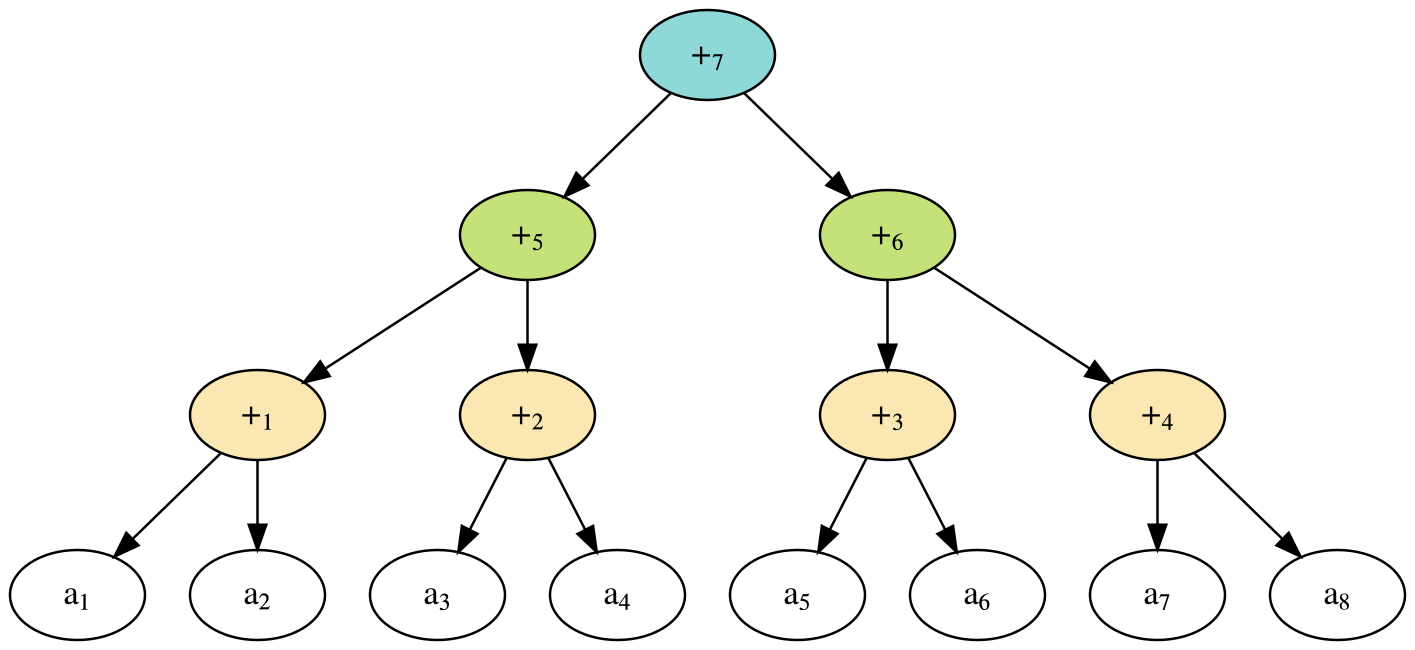
\includegraphics[height=4cm]{.dot/fold-parallel-2.png}
\end{center}

Every expression on each level does not depend on other expressions from the
same level, which means that we can evaluate them in parallel.
\end{frame}

\begin{frame}[label={sec:org784e9f1},fragile]{MapReduce}
 \begin{itemize}
\item <1-> Sometimes we have a collection of elements that don't form Monoid.
\item <2-> But we can transform (e.g. \texttt{map}) them into something that is a Monoid
\item <3-> There is a strange accent, where people pronounce 'fold' as 'reduce'.
\item <4-> This is how we get the \texttt{mapReduce}.
\item <5-> Just think about it, \texttt{mapReduce} is possible thanks to \texttt{Monoid} and its
\emph{laws}.
\end{itemize}
\end{frame}

\begin{frame}[label={sec:org7bc6731},fragile]{Coding time}
 \begin{itemize}
\item <1-> Our goal is to find 10 top used words among multiple books.
\item <2-> Open \texttt{wax.exercise.mapreduce.MapReduce} file.
\item <3-> \texttt{MapReduce} object implements \texttt{mapReduce} function (two variants - par and
seq).
\item <4-> \texttt{Main} object runs (not yet defined) \texttt{job} and profiles it (par vs seq).
\item <5-> \texttt{Result[Int]} is a map with words and their usage counter.
\item <6-> Your goal is to:
\begin{enumerate}
\item Implement monoid instance for \texttt{MapReduce.Result[Int]}.
\item Implement the \texttt{job} function to find the most used word.
\end{enumerate}
\item <7-> Use helpers from \texttt{FileUtils}:
\begin{itemize}
\item \texttt{readTokens} to get the list of words from the file.
\item \texttt{authorBooks} to get the list of books (files) by author (e.g.
\texttt{authorBooks("boris")}).
\item \texttt{allBooks} to get the list of all book among all available authors.
\end{itemize}
\end{itemize}
\end{frame}

\begin{frame}[label={sec:org17b8900},fragile]{Benchmarks}
 \begin{verbatim}
Par
duration = 65633 ms
result   = List(..., (people,37798), ...)

Seq
duration = 396530 ms
result   = List(..., (people,37798), ...)
\end{verbatim}
\end{frame}

\begin{frame}[label={sec:org990d224},fragile]{Outcome}
 \begin{itemize}
\item <1-> Thanks to \emph{associative} and \emph{identity} laws it's possible to implement a
parallel fold.
\item <2-> This is what makes \texttt{mapReduce} possible.
\item <3-> Many applications: inverted index, document clustering, machine learning.
\item <4-> Google used it to regenerate index of World Wide Web.
\end{itemize}
\end{frame}

\begin{frame}[label={sec:org06e29ff},fragile]{Homework}
 \texttt{mapReduce} is really interesting!

\pause

So play with it after the forkshop.
\end{frame}

\section{Logger}
\label{sec:org93a4a37}

\begin{frame}[label={sec:org996275a}]{Many monoids}
We dealt with some trivial monoids here:

\begin{itemize}
\item Integers with addition.
\item Strings and lists with concatenation.
\item Matrix with multiplication.
\item Maps of monoid values with merging.
\end{itemize}

\pause

They say that functional programming is all about \emph{functions}.

\pause

Can function be monoid?
\end{frame}

\begin{frame}[label={sec:orga9f97d3},fragile]{Let's start with some wrappers (pun intended)}
 \begin{itemize}
\item <1-> Suppose that we have some case class \texttt{Wrapper[A](value: A)}
\item <2-> Can it be a monoid?
\item <3-> Well, generally speaking, not! Because we know nothing about the type \texttt{A}.
\item <4-> But what if \texttt{A} is a monoid?
\item <5-> Hell, yeah!
\begin{minted}[]{scala}
case class Wrapper[A](value: A)

object Wrapper {
  implicit def wrapperMonoid[A: Monoid]: Monoid[Wrapper[A]] = new Monoid[Wrapper[A]] {
    override def empty: Wrapper[A] = Wrapper(Monoid[A].empty)

    override def combine(x: Wrapper[A], y: Wrapper[A]): Wrapper[A] =
      Wrapper(Monoid[A].combine(x.value, y.value))
  }
}
\end{minted}
\end{itemize}
\end{frame}

\begin{frame}[label={sec:org0f5149a},fragile]{Wrappers of monoids are monoids}
 \begin{itemize}
\item <1-> Since \texttt{IO} is a wrapper (in some sense), it \texttt{IO} can also be a monoid.
\begin{minted}[]{scala}
def ioMonoid[A: Monoid]: Monoid[IO[A]] = ???
\end{minted}
\item <2-> Which means that we can combine IO actions (in some new sense).
\item <3-> Functions are wrappers (in some sense), so they also can be monoids
\begin{minted}[]{scala}
def functionMonoid[A, B: Monoid]: Monoid[Function[A, B]] = ???
\end{minted}
\item <4-> Which means that we can combine functions (in some new sense).
\end{itemize}
\end{frame}

\begin{frame}[label={sec:org58e045b},fragile]{Logger}
 \begin{itemize}
\item <1-> What is logger?
\item <2-> \texttt{Logger} is basically a function from \texttt{String} to \texttt{IO[Unit]}.
\begin{minted}[]{scala}
type Logger = String => IO[Unit]
\end{minted}
\item <3-> \texttt{Unit} forms a monoid.
\item <4-> So \texttt{IO[Unit]} forms a monoid.
\item <5-> So \texttt{String => IO[Unit]} forms a monoid.
\item <6-> So \texttt{Logger} forms a monoid.
\item <7-> So we can combine loggers
\begin{itemize}
\item \texttt{fileLogger |+| consoleLogger} - logs both into file and to console
\end{itemize}
\end{itemize}
\end{frame}

\begin{frame}[label={sec:org9ac13c1},fragile]{Logger}
 \begin{minted}[]{scala}
def consoleLogger: IO[Logger] = IO { input =>
    IO {
      print(input)
    }
  }
\end{minted}

\pause

\begin{minted}[]{scala}
def fileLogger(filePath: String): IO[Logger] = IO {
  val stream = new FileOutputStream(filePath)
  input => IO(stream.write(input.getBytes))
}
\end{minted}

\pause

\begin{minted}[]{scala}
val program: IO[Unit] = for {
  logger <- consoleLogger |+| fileLogger("logging.log")
  _      <- logger("I am the log")
} yield ()
\end{minted}
\end{frame}

\begin{frame}[label={sec:org807c58b},fragile]{Logger}
 \begin{itemize}
\item <1-> Open \texttt{wax.exercise.logging.Logging} object.
\item <2-> Fill missing implementations.
\item <3-> Make sure to run \texttt{LoggingSpec} and make it green.
\item <4-> Run \texttt{Main} to see it in action.
\item <5-> Check \texttt{logging.log} file in the root of the project.
\item <6-> Have fun!
\end{itemize}
\end{frame}

\begin{frame}[label={sec:org609fe6d},fragile]{Bonus questions}
 \begin{itemize}
\item <1-> Is it possible to define several different semigroups for function?
\item <2-> What about monoids?
\item <3-> What about \texttt{Unit}?
\end{itemize}
\end{frame}

\begin{frame}[label={sec:org3c83439},fragile]{Outcome}
 \begin{itemize}
\item <1-> If you have a monoid, it's easy to form a new monoid (of a higher rank).
\item <2-> Function can also be monoid. This is really cool by itself.
\item <3-> Some of you probably gonna write new \texttt{colog} lib (but for Scala).
\end{itemize}
\end{frame}

\section*{Final words}
\label{sec:org7ecf94f}
\begin{frame}[label={sec:org9fae935},fragile]{Recap (recup?)}
 \begin{itemize}
\item <1-> Semigroup is something with means of combining these somethings.
\item <2-> Monoid is semigroup that also has neutral element that doesn't affect a combination.
\item <3-> Laws are really important.
\item <4-> Associativity is a powerful property giving us an ability to solve some tasks.
\begin{itemize}
\item \(a^n\) in \(\log n\)
\item \texttt{mapReduce}
\end{itemize}
\item <5-> Monoids are everywhere. They act like a plague, once something forms a monoid,
something else also begins to form a monoid.
\item <6-> We want some rest after a long session of forkshop.
\end{itemize}
\end{frame}

\section{Questions?}
\label{sec:orgbb7c8e4}

\section{Thank you very much!}
\label{sec:orgea5e389}
\end{document}
